\chapter{Layout}\label{chap:layout}

本章介绍数据库中常见的存储布局layout，包括关系数据库、kv数据库的存储布局。

\section{存储介质}

在组成原理的课程中，计算机体系结构中的存储介质呈现金字塔结构，从上到下分别是：寄存器、缓存、主存、硬盘等，如\figurename\ref{fig:2-pyramid}所示。数据是数据库最重要的资产，数据是保存在持久化介质中。

\begin{figure}[H]
    \centering
    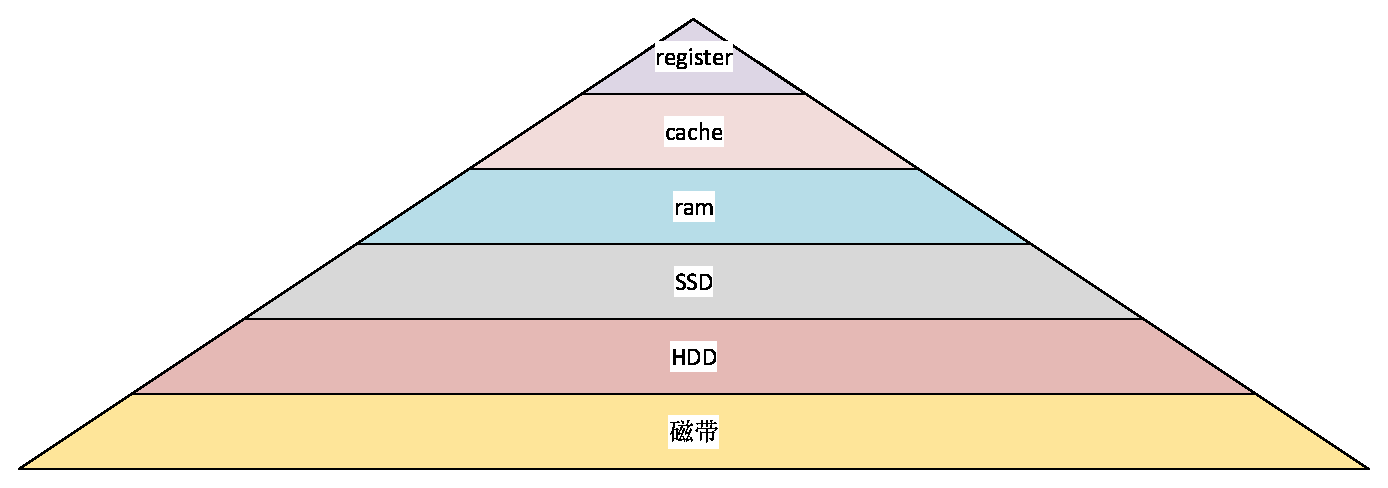
\includegraphics[width=\linewidth]{handout/img/2-pyramid.eps}
    \caption{存储介质金字塔结构}\label{fig:2-pyramid}
\end{figure}

\subsection{HDD}

传统的HDD硬盘，采用机械结构定位磁头，磁头以磁臂的轴心滑动，磁盘高速旋转在磁头感应出微弱信号，信号经过放大，转换为电信号，磁盘控制器通过DMA传送到内存，由CPU接手操作。

\begin{figure}[H]
    \centering
    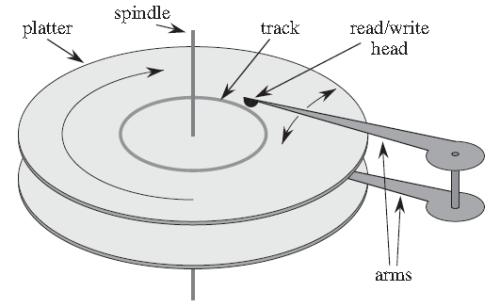
\includegraphics[width=0.5\linewidth]{handout/img/2-hdd.png}
    \caption{HDD硬盘机械结构}\label{fig:2-hdd}
\end{figure}

HDD盘片的双面喷涂磁性材料，这样就需在盘片上下布局磁头。同时，为了增加磁盘容量，会串接多个盘片。每个盘的表面，都有多个磁道，每个磁道上有多个扇区，如\figurename\ref{fig:2-sector}所示。多个磁头的磁臂被固定在一起，当磁臂滑动，所有磁头都滑动到相同位置上。这样，多个盘片的同心磁道组成了一个柱面cylinder。

磁盘的传输单位是扇区sector，通常每个扇区512B。传统HDD硬盘，为定位一个扇区，采用柱面-磁头-扇区3D(Cylinder-Head-Sector)方式定位。这种3D定位方式与厂商的实现有关，不同厂商可能采用不同的方式。为了简化BIOS实现，现代HDD硬盘，通常采用LBA(Logical Block Address)方式定位扇区。LBA方式将柱面-磁头-扇区3D定位方式，映射为一个线性地址，这样就可以用一个简单的整数来定位一个扇区。

\begin{figure}[H]
    \centering
    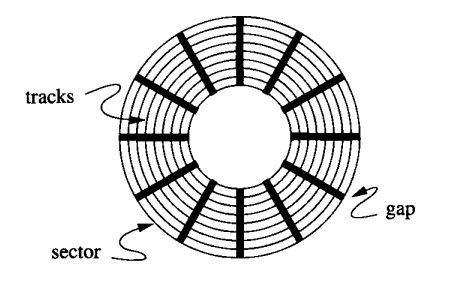
\includegraphics[width=0.6\linewidth]{handout/img/2-sector.png}
    \caption{HDD扇区}\label{fig:2-sector}
\end{figure}

由于HDD硬盘读写采用机械结构定位磁头，寻道时间比较长，一般在10ms左右，旋转延迟一般在5ms左右。传输延迟是将数据从磁盘传送到内存的时间，由于是电信号，延迟很小。

为了加速HDD访问，一般有几种方案：设置缓冲，电梯算法，临近存放，RAID并行等。

\begin{exercise}
    证明磁头的平均移动距离是总距离的1/3。
\end{exercise}
\begin{exercise}
    一般文件系统以block为单位提供存储服务，每个block包括多个扇区，通常为4KB。文件系统声称一个操作是原子的，是指这个操作很快吗？如果不是，那是指的什么？
\end{exercise}
\begin{exercise}
    journal文件系统是一种日志文件系统，它将所有修改操作记录在日志文件中，然后再进行实际的修改。这样可以避免在修改过程中发生故障，导致数据丢失。它是如何实现原子操作的？
\end{exercise}

\subsubsection*{临近存放}

假设一个文件比较大，文件会包含多个扇区。一般文件系统管理磁盘的时候，随着文件增大，按需分配扇区。如果不采取措施，这个文件的扇区会随机分别在磁盘上，IO开销会很大。并且，随着系统运行时间增加，通常而言，磁盘上的文件组织呈现碎片化，有些文件系统会在后台尝试整理硬盘，挤压碎片。

临近存放的策略是，每次文件增长时，申请足够多的扇区数目，文件系统一般会顺序在磁盘上分配，这些分配的扇区会以很高的概率分配在临近的柱面上。如前所述，所有磁头是同步固定的，这样一来就节省了寻道时间。

\begin{exercise}
    Google的文件系统GFS，它每次分配文件都按照一个chunk为单位，每个chunk默认是64MB。解释一下，这种策略的优势。
\end{exercise}

\subsubsection*{RAID}

RAID(Redundant Arrays of Independent Disks)冗余磁盘阵列将多个物理磁盘组合成一个逻辑磁盘，提供数据冗余和性能提升。标准规定了RAID 0-5，RAID 6由厂商自定义。

\begin{exercise}
    查找资料，学习RAID 0-5，RAID 6的原理，包括条带化、镜像、校验、均衡等手法。
\end{exercise}

HDD受限于机械结构，IO访问时间一般平均在10ms左右，相比于CPU执行执行，非常慢。现代CPU执行一条指令平均在2ns左右，两者相比，HDD的IO访问时间是CPU执行指令的100,000-1,000,000倍。所以，在数据库领域，衡量数据库性能，一般计算对HDD硬盘的访问次数就够了。

\begin{figure}[H]
    \centering
    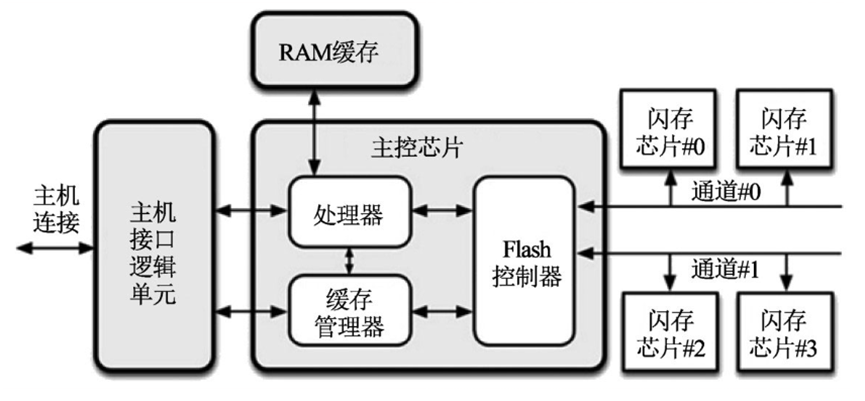
\includegraphics[width=0.8\linewidth]{handout/img/2-ssd.png}
    \caption{SSD内部结构}\label{fig:2-ssd}
\end{figure}

\subsection{SSD}

随着SSD硬盘的普及，目前大量数据库系统采用SSD硬盘作为存储设备。SSD设备没有机械结构，使用支持NVMe协议的M.2接口的随机读写速度一般都在1000KIOPS之上，延迟一般在250us左右。相比于CPU指令执行，SSD的IO访问时间是CPU执行指令的50,000-100,000倍左右。

SSD内部基本上是一个mini的计算机系统，从PCIe通道发送来的速写指令传递到SSD，SSD内部会解析指令，根据指令进行数据读写。SSD内部有多个NAND flash内存芯片，每个芯片有多个页page，每个页有多个块block，每个块有多个扇区sector。SSD内部有一个控制器，负责接收指令，解析指令，根据指令进行数据读写。

SSD的NAND flash器件，与硬盘的读写特性不一样，它有三种操作：读、写和擦除。读写操作是将数据从内存写入NAND flash，或者从NAND flash读取数据到内存。擦除操作是将NAND flash上的一个块全部擦除，变成未写状态。三种操作的耗时是不同，读最快，写大约比读慢10倍，擦除大约比读慢100倍。

\begin{table}[H]
    \centering
    \caption{HDD与SSD性能对比}
    \label{tab:2-hdd-ssd-comparison}
    \begin{tabularx}{\linewidth}{lXXX}
        \toprule
        \textbf{指标} & \textbf{HDD（机械硬盘）} & \textbf{SSD（固态硬盘）} & \textbf{倍数（近似）} \\
        \midrule
        顺序读取带宽 &
        \begin{minipage}[t]{\linewidth}
            100～200MB/s
        \end{minipage} &
        \begin{minipage}[t]{\linewidth}
            7,000MB/s
        \end{minipage} &
        \begin{minipage}[t]{\linewidth}
            70倍
        \end{minipage} \\

        随机读取 IOPS &
        \begin{minipage}[t]{\linewidth}
            50～150 IOPS
        \end{minipage} &
        \begin{minipage}[t]{\linewidth}
            10,000～1,000,000+ IOPS
        \end{minipage} &
        \begin{minipage}[t]{\linewidth}
            100～10,000 倍
        \end{minipage} \\

        访问延迟 &
        \begin{minipage}[t]{\linewidth}
            5～15 毫秒（ms）
        \end{minipage} &
        \begin{minipage}[t]{\linewidth}
            0.01～0.1 毫秒（即 10～100 微秒）
        \end{minipage} &
        \begin{minipage}[t]{\linewidth}
            约 50～1,000 倍
        \end{minipage} \\
        \bottomrule
    \end{tabularx}
\end{table}

SSD盘为了兼容HDD的文件接口，会在SSD内部实现Garbage Collection机制，对block的修改会先写入到一个空闲的block中，然后将原来的block标记为已删除。当SSD内部的block被写满后，会触发垃圾回收，将已删除的block中的数据复制到新的block中，释放空间。

SSD的GC与文件系统在功能上存在语义重叠，二者工作在不同层次、缺乏协同，因信息不对称导致效率损失。例如，文件系统的空闲对SSD是不可见的：
\begin{enumerate}
    \item 用户删除一个1GB文件 $\rightarrow$ 文件系统在元数据上标记 LBA [1000–2000] 为空闲。
    \item SSD并未收到回收这些LBA的通知，仍然认为这些LBA的物理页是有效数据，因此不会被回收。
\end{enumerate}
现代系统引入跨层通信协议，文件系统在删除文件后，向 SSD 发送 TRIM 命令，告知：“LBA X–Y 已不再使用”。SSD 的 FTL 将这些 LBA 对应的物理页标记为“无效”。更新的方案是将SSD的GC机制与文件系统的空闲管理机制进行整合，将SSD的部分功能上移到文件系统，使其能够直接管理物理块。

\begin{exercise}
    查找ZNS SSD / Open-Channel SSD资料，了解跨层文件系统整合方案。
\end{exercise}
\begin{exercise}
    在HDD上，采用预分配大块连续LBA的方案，利用临近柱面寻道事件短的优势，提高IO性能。查找SSD的相关资料，基于SSD并行访问的物理构架，能否提出一种LBA预分配方案，提升IO读写性能。
\end{exercise}

\section{数据库文件}

数据库管理系统一般包括数据文件、索引文件、日志文件、元数据文件、配置文件等。这些文件的通途不同，访问模式也不同。数据文件用于存储tuple数据，关系型数据库的数据文件通常是分页的，索引文件的结构一般与数据文件类似。日志文件用于记录数据库的操作，以便在系统故障时进行恢复，它的操作一般是追加。元数据文件用于存储数据库的结构信息，例如表、索引、约束等，很少修改。配置文件用于存储数据库的配置参数，例如缓存大小、IO 调度策略等，更少修改。

\begin{figure}[H]
    \centering
    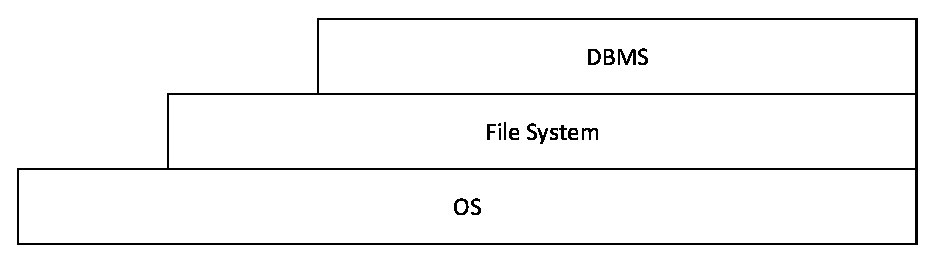
\includegraphics[width=0.8\linewidth]{handout/img/2-dbms.eps}
    \caption{数据库与文件系统}\label{fig:2-dbms}
\end{figure}

大多数数据库管理系统会以文件作为存储单位，将数据文件、索引文件、日志文件、元数据文件、配置文件等存储在不同的文件中，如\figurename\ref{fig:2-dbms}所示。极少数软硬件通吃的厂商会将DBMS直接集成在操作系统中，让DMBS直接管理HDD/SSD等存储设备。

\begin{figure}[H]
    \centering
    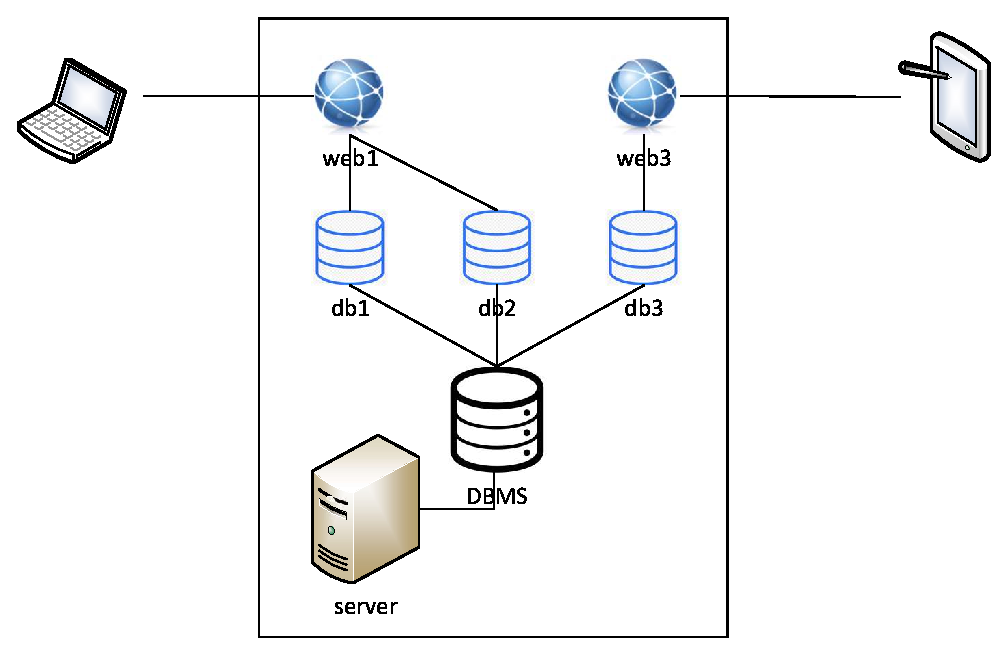
\includegraphics[width=0.9\linewidth]{handout/img/2-deploy.eps}
    \caption{数据库部署}\label{fig:2-deploy}
\end{figure}

在DBMS中，一般假设，一个关系对应于一个数据或多个数据文件，很少会将一个数据文件用于存储多个关系。最简单的方案是每表一文件，即规定每个关系对应于一个数据文件。但复杂构架下的数据库，数据文件可能跨节点分布式存储，一个关系可能对应于多个文件。

DBMS部署一般的模型如\figurename\ref{fig:2-deploy}所示，一个DBMS实例对应于一个物理节点，一个DBMS实例可以运行多个数据库实例。Oracle比较特别，它不支持CREATE DATABASE，每个用户拥有自己的Schema，而不是数据库实例。

考虑到存储的异质，HDD/SSD它们的特性完全不同，PostgreSQL引入表空间概念，用一个目录表示特定存储设备，表的数据文件可以存在不同的表空间中，一个表空间也可以容纳多个表的数据文件。Innodb/Oracle则不同，它们的表空间概念是逻辑上的，一张表对应于一个表空间，表空间容纳多个该表的数据文件。

\subsection{分页}

考虑一个Relation如何将它的tuple存放在一个文件中。最简单的模型，将文件看成一个连续堆，tuple直接顺序写入文件。这种模型简单直接，但是tuple可能会修改删除，从而导致文件碎片化，降低IO性能。

\begin{figure}[H]
    \centering
    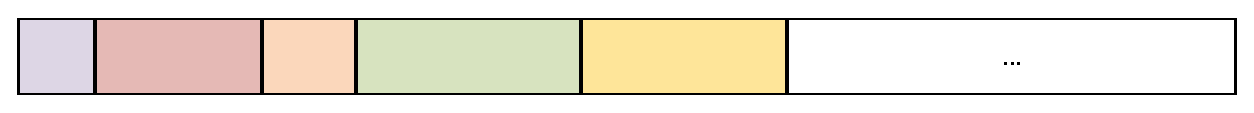
\includegraphics[width=0.8\linewidth]{handout/img/2-heap.eps}
    \caption{简单的堆模型}\label{fig:2-heap}
\end{figure}

操作系统的内存管理可以分段、分页，将物理内存分成固定大小的页，小内存从页面上分配，碎片化仅在页内，不会影响整体性能。借鉴这种思路，数据库的文件管理也可以采用分页的方式，将文件分成固定大小的页，tuple存放在页内。

\begin{figure}[H]
    \centering
    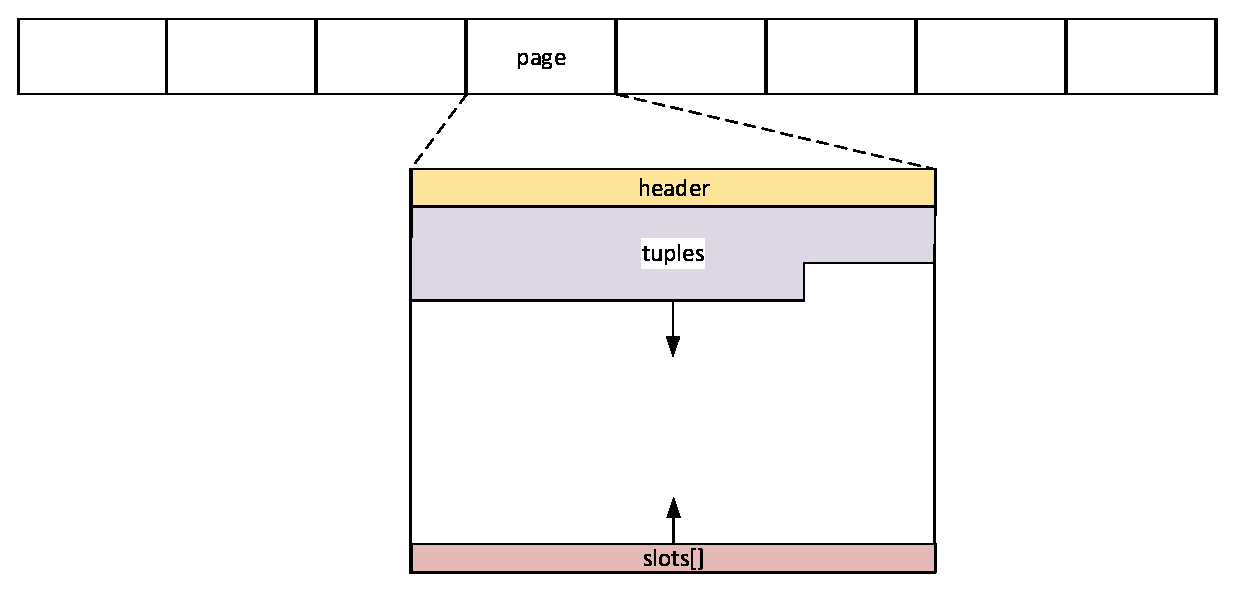
\includegraphics[width=\linewidth]{handout/img/2-page.eps}
    \caption{数据文件分页模型}\label{fig:2-page}
\end{figure}

按照\figurename\ref{fig:2-page}所示，数据文件按照page大小分页存储，每个页包含多个tuple。为管理页面内部的tuple，页面有特定格式，前部是固定大小的头部header，然后是tuple载荷，页面的后部是slots[]数组。slots[]数组用于记录每个tuple的偏移量和大小，方便数据库管理系统快速定位和访问tuple。tuples和slots大小可变，因此分别位于空闲区域的上下两侧，从两个方向扩展。

数据文件分页后，数据库可以管理自己的缓冲，由于页面大小固定，数据库的缓冲设计相对简单。相对于OS缓冲，数据库更了解这些页面的用途，哪些页面可以直接drop掉，哪些页面需要回写。而OS内核缓冲由于难以获取这些信息，缓冲效率较低。

\begin{exercise}
    操作系统一般配置了虚拟内存，当物理内存不敷使用时，会将一部分内存分页转储到硬盘上，称为交换空间。分析一下，当数据库系统进程切换时，数据库的页面是否会被放到交换空间中？如果会，会有什么影响？
\end{exercise}
\begin{exercise}
    数据库日志文件一般会以O\_APPEND模式打开，即每次写入日志时，会将数据追加到文件末尾，而不是覆盖原有内容。Linux系统将这种写入称为原子的，追加写入是否安全？有何风险？
\end{exercise}
\begin{exercise}
    Innodb的数据文件每次扩容，按照extend机制增长，extend最初为8MB，后续会动态增加到64MB。Innodb为什么会引入extend机制？
\end{exercise}

\subsection{分段}

数据文件分页，其设计目标主要是为了容纳tuple，减少碎片化，提升性能。除了容纳tuple外，数据文件其实还有更多的需求，如垃圾收集、容纳BLOB等、维持多版本、构建索引等。

在数据文件内部分段，是基于功能的考虑：存储tuple的数据段、构建索引的索引段、容纳BLOB的溢出段、维持旧版本的堆段。数据文件内的页面根据功能和用途，被划分的不同的逻辑段。

\subsubsection*{超块}

数据文件的头部一般存储该数据文件的一些元信息，包括文件大小、空闲链表指针等，本文称为超块superblock。超块的目的是为了描述该数据文件，给出数据文件内部各段的起始位置和大小等信息。

\begin{figure}[H]
    \centering
    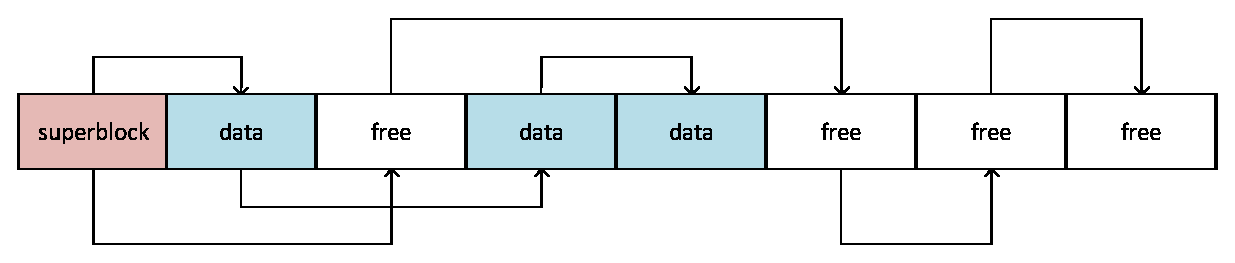
\includegraphics[width=\linewidth]{handout/img/2-superblock.eps}
    \caption{超块页面}\label{fig:2-superblock}
\end{figure}

\begin{exercise}
    超块用于描述数据文件，为了防止对超块的写入错误，超块该如何设计？采用日志，描述超块的修改操作？或者使用双超块？
\end{exercise}

\subsubsection*{垃圾收集与空闲链表}

btree在合并页面后，会废弃一些旧的页面，这些页面被称为空闲页面，空闲页面会被加入到空闲链表中。数据文件在增长时，也会出现空闲页面，这些页面会被加入到空闲链表中。空闲页面以单向链表的形式组织，每个页面包含一个指向下一个空闲页面的指针，如\figurename\ref{fig:2-superblock}。

\begin{exercise}
    为什么不采用双向链表组织空闲页面？或者其它结构？
\end{exercise}

\begin{exercise}
    数据文件如果部署在SSD，该如何管理空闲页面？采用前述的空闲链表，显然有问题。写入后继指针意味着该页面脏，当重新启用该空闲页面，SSD控制器需要从内部的干净页面上再分配来替换这个空闲页面。该用什么方案来解决这个问题？
\end{exercise}

\subsubsection*{溢出页面}

当tuple对应的record尺寸超过页面大小，会发生溢出。溢出部分需要存放在其余页面中，这些页面称为溢出页面。异常页面的头部仍然是固定大小的，与普通数据页面格式相同，只是slots数组可以不再需要。溢出页面需要专门的段来容纳？不需要，它是普通页面的附属。

\begin{figure}[H]
    \centering
    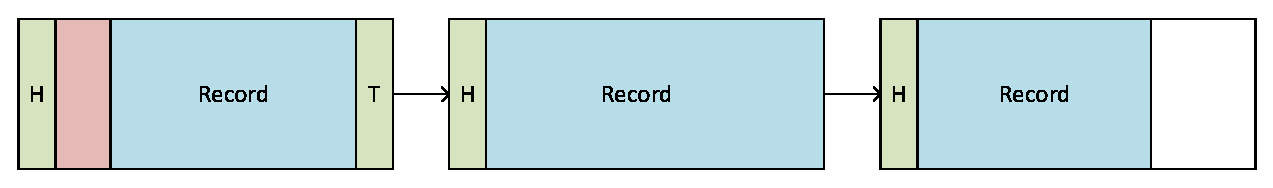
\includegraphics[width=\linewidth]{handout/img/2-blob.eps}
    \caption{溢出页面}\label{fig:2-blob}
\end{figure}

\subsubsection*{旧版本/undo页面}

在MVCC并发控制的数据库系统中，如PostgreSQL/Oracle等，每个key对应于多个版本，版本之间通过时间戳区分，以单向链表形式组织。有些MVCC系统，将旧版本存放在单独的旧版本页面中，而不是与当前版本页面混合在一起。原因是当前版本一定是访问最多的，旧本部访问概率较小，数据页面容纳的record会更多，有助于提升性能。

旧版本页面一般采用堆模型，不会再聚集，这是后面的聚集存储的知识，这里先提一句。旧版本页面一般采用单向链表组织，构成一个段。

\section{Record}

逻辑上，Relation由tuple构成，每个tuple包含多个字段，每个字段有特定的类型。在数据库层面，由于创建的表各不相同，每个关系的tuple字段数量和类型也不同。存储在页面上的tuple，有特定的格式，而不能是简单的字段序列。为区分逻辑上的tuple，将页面上存储的tuple称为记录record，记录带有一定的格式，根据这个格式能够区分出各个字段的长度。

\subsection{记录格式}

站在数据库的角度，记录中字段类型和长度是变化的，完全依赖于Schema不可行。例如，一个变长字符串VarChar(10)，它是说这个字段最长10B，字段长度是不定的，如果在记录中保留10B空间，会使得存储效率低下，IO效率也会降低。因此，记录需要有一定的自解释能力。

记录格式的设计基本要求是能够描述各字段的长度，各数据库的设计有很大不同，这里给出的设计参考了Innodb的方案，但与之稍有不同。如\figurename\ref{fig:2-record}所示，记录主要包含以下几个部分：

\begin{itemize}
    \item header，定长，包含记录的一些元信息，tomstone标记，溢出标记等。
    \item total，变长，记录完整长度。
    \item offsets，变长数组，记录中所有字段的偏移量，偏移量从offsets结尾开始计算，每个偏移量仍然是变长整数。
    \item fields，变长数组，记录中所有字段的实际数据，每个字段的长度根据offsets中描述的偏移量和下一个偏移量之间的差值确定。最后一个字段的长度，需要total参与计算。
    \item pads，填充为0，对齐8B。
\end{itemize}

\begin{figure}[H]
    \centering
    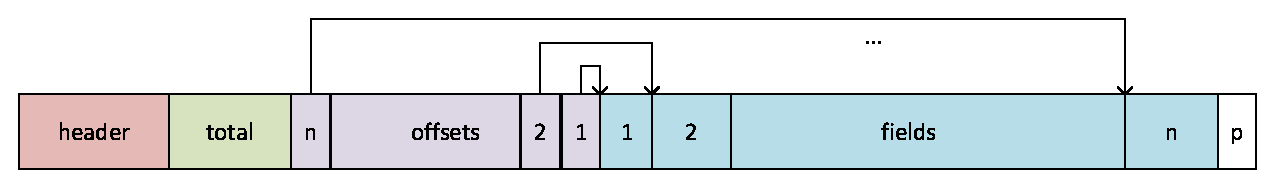
\includegraphics[width=\linewidth]{handout/img/2-record.eps}
    \caption{记录格式}\label{fig:2-record}
\end{figure}

整个记录的设计要点是，使用各字段的offset来计算字段的长度，offsets按照逆序排列，第1个字段的offset排在最后且为0。这样offsets数组虽然每项都是变长的，数目也不确定，但是数值是单调递减到0，从而能够识别出整个offsets数组，不需要Schema的参与。

Innodb中，记录中保存的是各字段的长度，虽然也是逆序保存，但并不象offset一样具有单调性，必须依赖Schema指示字段个数。

\begin{figure}[H]
    \centering
    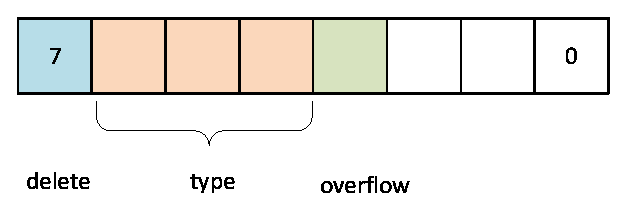
\includegraphics[width=0.5\linewidth]{handout/img/2-header.eps}
    \caption{记录头格式}\label{fig:2-header}
\end{figure}

记录的头部长度固定，暂定为1B，bit7表示tomestone标记，bit6-4是类型标记，bit3表示溢出标记，最低3bit保留。记录类型用于标记是何种类型，有些记录可以使用各种压缩方案。

\subsection{溢出记录}

溢出记录会跨页面保存，如\figurename\ref{fig:2-blob}所示。为响应溢出需求，在记录的header后部添加next字段，该字段定长，指向记录存储的下一个页面。如\figurename\ref{fig:2-overflow}，page2如果放不下，会继续分配页面容纳溢出记录，后续页面之间通过后继指针连接。next字段后是变长的first字段，它指明记录在该页面中的存放大小。next/first字段要尽可能排列在记录的前部，以避免从这两个字段被截断。

溢出记录在截断时，按照8B对齐，不填充。

\begin{figure}[H]
    \centering
    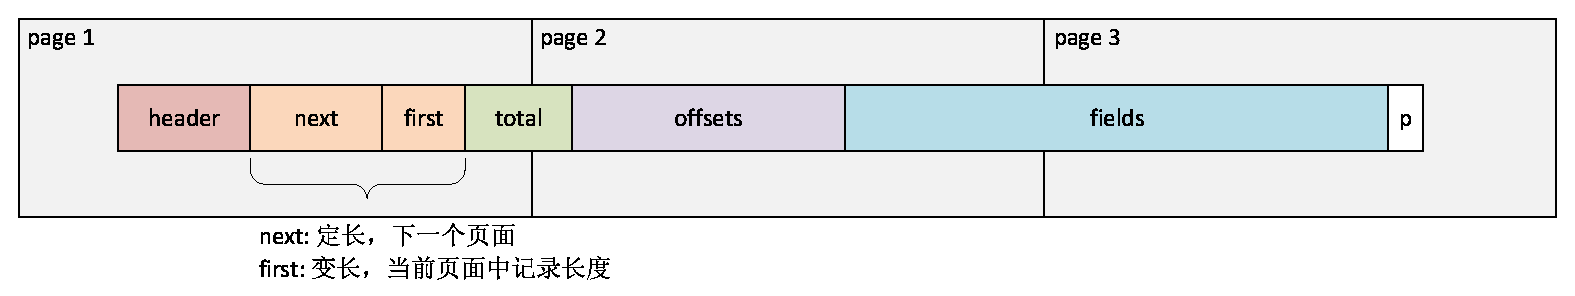
\includegraphics[width=\linewidth]{handout/img/2-overflow.eps}
    \caption{溢出记录跨页面保存}\label{fig:2-overflow}
\end{figure}

\subsection{xmin/xmax}

在PostgreSQL这样的堆存储方案中，由于支持MVCC，一般会在记录中添加xmin/xmax字段，用于记录该记录的可见性。xmin表示该记录被哪个事务创建，xmax表示该记录被哪个事务删除。如\figurename\ref{fig:2-mvcc}，根据key找到记录的位置，然后从page上的slots定位到record1，这是最初的版本。所有版本一般会临近存放，按照从旧到新顺序指向。

\begin{figure}[H]
    \centering
    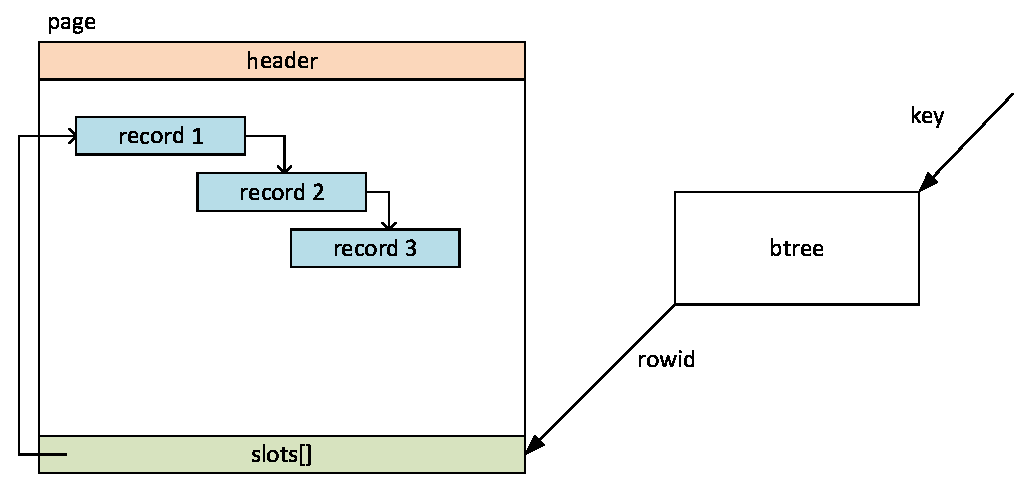
\includegraphics[width=\linewidth]{handout/img/2-mvcc.eps}
    \caption{PostgreSQL多版本存储}\label{fig:2-mvcc}
\end{figure}

在PostgreSQL的非聚集存储方案中，rowid并非是tuple的id，它是一个复合整型：利用某些位来表示页面号，利用其他位来表示的slots序号。拿到rowid后，会先找到对应的页面，然后再根据slots序号找到记录的offset，从而定位到记录。由于存在多个版本，为了快速定位到对应的版本，PostgreSQL的记录格式使用定长xmin/xmax，不需要打开记录格式，能够快速定位记录。

与PostgreSQL不同，Innodb是聚集存储，key临近的记录会聚集在临近的页面。但Innodb页面的slots需要按照key排序，这需要打开记录访问key。PostgreSQL中，btree指向的rowid一般是不动的。而innodb中，btree只需给出记录所在的页号，但页面插入一个记录后，该页面有可能分裂，导致btree指向的页号发生变化。——这是不同的设计选择带来的。

与PostgreSQL不同，Oracle的btree则指向最新的记录，新记录指向旧记录，与PostgreSQL刚好相反。旧记录并不就近保存，而是在旧版本段内维护。

\subsection{rowid}

rowid在堆存储模型中非常有用，它表示一条记录在数据库中的物理位置，用于快速定位一条记录，是一条记录的唯一标识符。rowid一般并不会暴露给用户，而是在系统内部使用。在聚集存储中，如innodb，一般直接使用key来定位记录，而不是rowid。

不同的数据库中，rowid的实现方式不同，甚至名字也不同。Oracle的rowid采用10字节存储，显示为18B的Base64字符串，格式如下：
\begin{lstlisting}[style=verbose]
OOOOOOFFFBBBBBBRRR
│     │   │     └─── Row number (3 chars) → 行在块中的位置（从 0 开始）
│     │   └───────── Block number (6 chars) → 数据块编号
│     └───────────── Relative file number (3 chars) → 相对文件号
└─────────────────── Data object number (6 chars) → 对象 ID
\end{lstlisting}

PostgreSQL的ctid与Oracle的rowid近似，它使用两个整型$[pageno, index]$表示一条记录：
\begin{itemize}
    \item pageno，int32，记录所在的页面编号。
    \item index，记录在页面中slots数组中的序号。
\end{itemize}

在实现中，rowid一般会采用变长表示，放在记录中，只有打开一条记录才能获取rowid。所以，不管是Oracle的rowid，还是PostgreSQL的ctid，不用担心rowid的长度问题。

在堆存储中，一般页面布局仍然采用\figurename\ref{fig:2-page}方式，只是页面尾部的slots数组不再是按照key排列，而是按照记录写入的先后顺序排列。这带来的问题是，如果删除一条记录，它的槽位会被保留，以免影响其它记录的定位。虽然损失的资源较小，后续可以安排一个扫描线程，回收这部分资源。

\section{kv存储}

传统关系型数据库主要使用btree作为索引，主要针对OLTP应用，这些应用一般要求读写平衡。21世纪以来，随着云计算、大数据的发展，大规模OLAP的应用需求逐渐占据主流地位，这些应用的特征是，采用批处理模型，批量写入而非更新，同时对读操作性能要求较高。在这种场景下，kv存储基于列存、无结构、IO效能较高，逐渐成为新型存储组织方式。

kv存储的需求主要来源于批处理场景，设想一下，源源不断的数据写入，如果使用传统的数据组织，还需要找到对应的位置插入，即使使用堆模型，也需将数据插入到结构化的页面中。最简单的方式是，将数据在内存里排好，当数据量超过一定阈值时，一把写入磁盘，也不用带什么页面格式。

\begin{figure}[H]
    \centering
    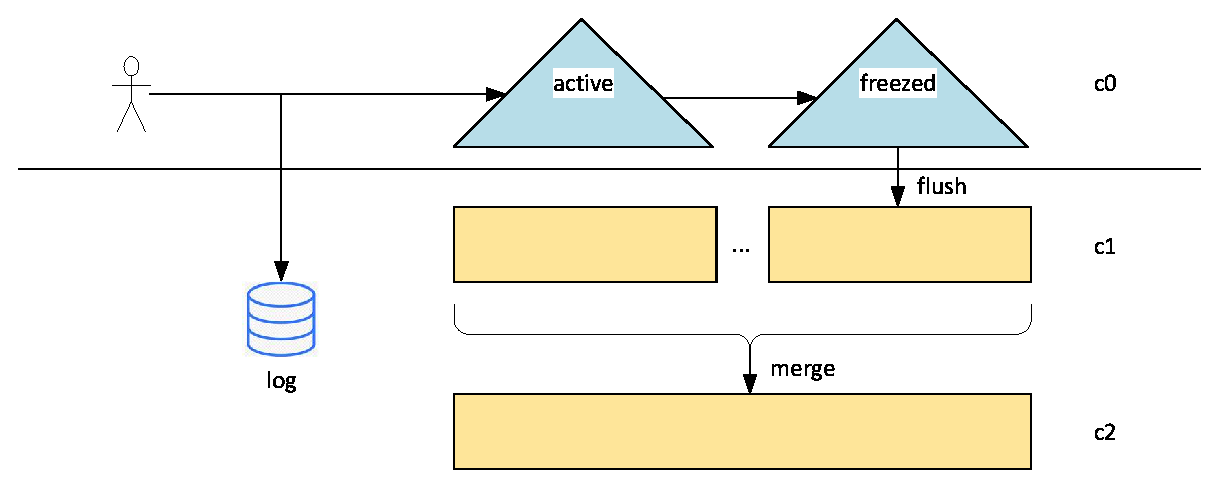
\includegraphics[width=\linewidth]{handout/img/2-lsm.eps}
    \caption{LSM-tree结构}\label{fig:2-lsm}
\end{figure}

LSM-tree\cite{o1996log}是这种思路的实现方案，数据到达，先写日志，然后在内存里排序，当容量超过阈值时，将这个排序结构凝固，然后flush到磁盘。按照这个方案，写入速度会极快，甚至在批处理场景下完全可以不写日志，出错后重启批处理即可。后面为了查询方便，启动一个后台进程，对写入数据做多路归并merge，将小块的有序数据规整为有序的更大块数据。

\subsection{leveldb存储格式}

leveldb\cite{GitHubgo38:online}是LSM结构的一个成熟实现，作者Jeff Dean在google有较长的工作经历，在从google退出后，开源了这个项目。leveldb是google多年kv存储开发经验的集大成作品，发布虽晚于HDFS，但它的成熟设计、高质量代码在发布后立即受到了广泛关注。

这里仅讨论leveldb的底层存储格式，它的架构留到下一章再介绍。

\begin{figure}[H]
    \centering
    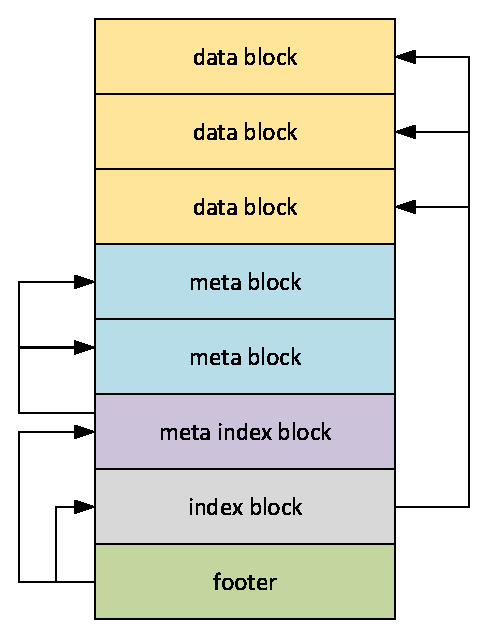
\includegraphics[width=0.5\linewidth]{handout/img/2-sstable.eps}
    \caption{sstable结构}\label{fig:2-sstable}
\end{figure}

leveldb将底层存储格式称为sstable，sstable的格式如\figurename\ref{fig:2-sstable}所示。它内部主要包含5个部分：

\begin{itemize}
    \item data block：存储实际的key-value数据记录。
    \item meta block：存储一些额外的元数据，如压缩算法、校验和等。
    \item index block：用于定位data block，给出每个data block的offset和size。
    \item meta index block：用于定位meta block，给出每个meta block的offset和size。
    \item footer：sstable访问入口，定长位于sstable文件尾部。
\end{itemize}

\begin{figure}[H]
    \centering
    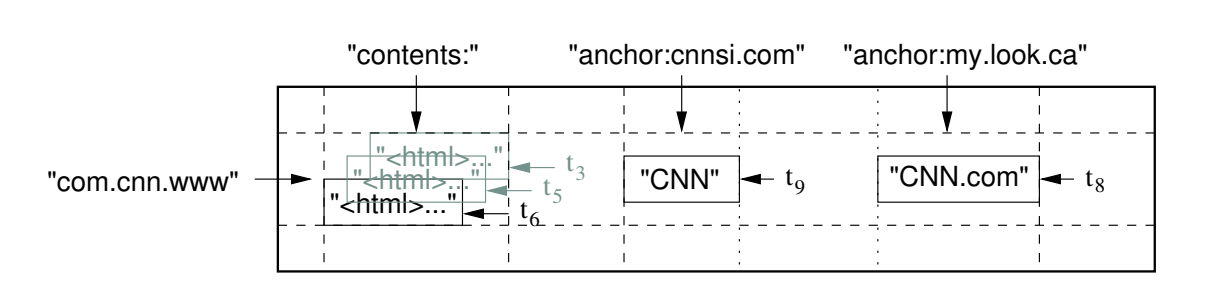
\includegraphics[width=\linewidth]{handout/img/2-kv.png}
    \caption{kv存储模型示例}\label{fig:2-kv}
\end{figure}

对sstable的访问是从尾部footer开始的，footer大小固定，内部有两个指针，分别指向meta index block和index block。如果寻找数据，则从index block开始，二分查找key所在的data block，然后从data block开始顺序查找。

sstable中，datablock和indexblock都是按照kv格式存储。kv存储的数据模型不再是关系型数据库的关系型模型，而是一种简单的键值对。kv模型相对于关系，它更简单，表达能力更强。以\figurename\ref{fig:2-kv}为例，批处理的爬回的页面以kv方式存储，url为www.cnn.com的页面，其网页内容存储在一个单元中。这个单元存放多个爬回的版本，这些版本以时间$t_3,t_5,t_6$作为key存储。这个例子中，anchor称为一个列族，按照锚点cnnsi.com、my.look.ca划分出不同的列，www.cnn.com对应的列族有不同的kv值。从这个例子来看，kv存储非常自由，列并不固定，允许嵌套。

\begin{exercise}
    如果用kv方式来存储一张关系表，采用列式存储，key可能重复多次写入。有没有可能采用key/value分离的方案，将表的一列分别存储？参考tdengine的存储模型提出解决方案。
\end{exercise}

sstable中的kv存储是将一列的多个kv对连续存储，这些kv对按照key顺序排列。由于key类型相同，并且临近kv对的key值相近，因此采用前缀压缩存储。每个kv对称为一个entry，在\figurename\ref{fig:2-prefix}中，key2要和前面的key1相比，表示共享了多少个字节，有多少字节的不同，然后给出不同部分以及value。

\begin{figure}[H]
    \centering
    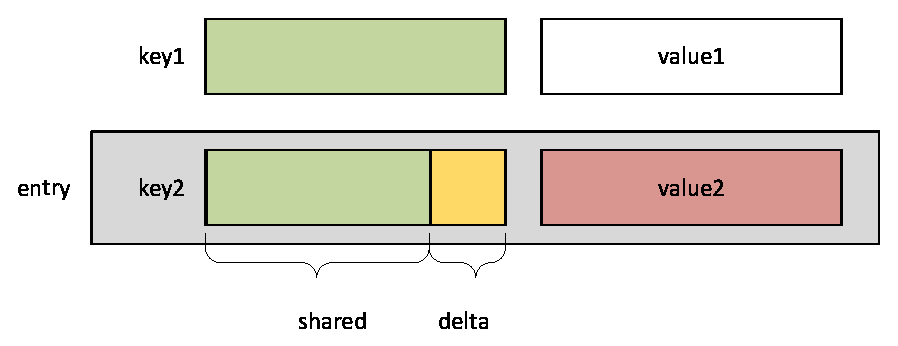
\includegraphics[width=0.8\linewidth]{handout/img/2-prefix.eps}
    \caption{kv前缀压缩示意图}\label{fig:2-prefix}
\end{figure}

leveldb在TableBuilder中创建一个sstable，datablock的格式如\figurename\ref{fig:2-block}所示。offset指向一个datablock，每个datablock的大小约为4KB，不一定对齐4KB。根据size找到datablock的尾部，尾部为num\_restarts、type、crc32，这几个字段都是固定大小。在num\_restarts之上是restarts[]数组，数组的每一项是固定大小的restart偏移量。

leveldb采用前缀压缩存储kv对，在TableBuilder构造datablock时，默认每16个kv对处理为一组，称为一个restart point。每个kv对的存储格式包含5个部分。shared\_bytes表示该kv对与restart point最前面的kv对共享的字节数，non\_shared\_bytes表示key中不同的字节数，value\_length表示value的长度，non\_shared\_key表示key中不同的部分，value表示value。

\begin{itemize}
    \item shared\_bytes (varint32): 表示key和前一个key共享的字节数。
    \item non\_shared\_bytes (varint32): 表示key中不同的字节数。
    \item value\_length (varint32): 表示value的长度。
    \item non\_shared\_key (bytes): 表示key中不同的部分。
    \item value (bytes): 表示value。
\end{itemize}

\begin{figure}[H]
    \centering
    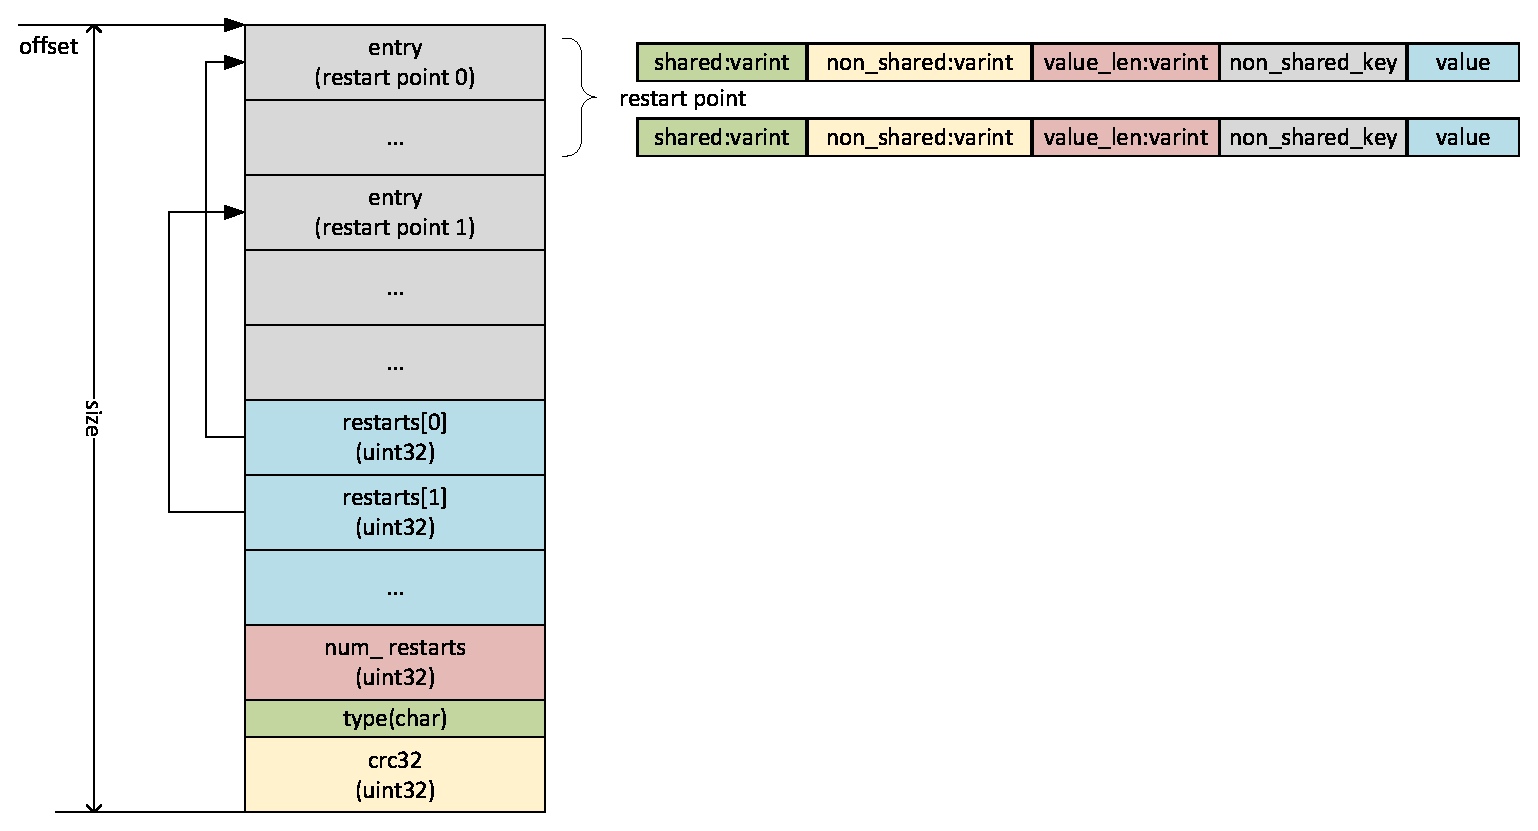
\includegraphics[width=1.2\linewidth]{handout/img/2-block.eps}
    \caption{data block格式}\label{fig:2-block}
\end{figure}

\begin{exercise}
    \figurename\ref{fig:2-block}展示的是datablock的格式，index block的格式呢？sstable中，indexblock可以有多个吗？sstable尾部footer，是否要包含indexblock的大小？
\end{exercise}
\begin{exercise}
    每个restart point最前面的kv对，key的shared\_bytes为多少？non\_shared\_bytes为多少？
\end{exercise}
\begin{exercise}
    关系型数据库中，一般在数据文件的头部放元信息。sstable中的footer包含元信息，为什么放在尾部？同样，num\_restarts也放在尾部，CRC32也放在尾部，这是为什么？
\end{exercise}
\begin{exercise}
    数据校验的方式有多种，有奇偶校验，crc校验，sstable为什么采用crc32？采用奇偶校验行不行？
\end{exercise}

整个datablock内存构建完成后，可以进一步使用snappy压缩，snappy压缩方案速度极快，压缩率中等。然后设置datablock尾部的type，表示为snappy压缩的block。

\section{实验}

本章设计三个实验，分别为聚集存储、堆存储和kv列式存储，前两个是关系型数据库的存储方案，最后一个是kv列式存储方案。

\subsection{聚集存储}

聚集存储实验主要参考innodb方案，数据文件分页，页面格式大致为\figurename\ref{fig:2-page}。聚集存储的页面，slots数组存放kv对的偏移量，这些偏移量按照key顺序排列，搜索以二分查找。使用key查找对应的记录，需要打开记录格式，比较key。

聚集存储的数据一般与主键索引合并存放，数据页面看成btree的叶子节点。每次新插入一条记录，可能会导致页面分裂，由于数据页面看成btree的叶子节点，数据页面分裂可能会引起btree调整。

以上是聚集存储相对于堆存储模型的劣势，但聚集存储带来的好处是，由于key相近的记录存放在相邻的页面，因此可以利用缓存预读，提高访问效率。也就是说，聚集存储以插入的代价换取了查找性能的提升。

\subsection{堆存储}

堆存储实验参考PostgreSQL的存储方案，堆模型将所有页面看成一个堆。当需要分配一个空闲空间，堆模型不会去按照key相近的原则去寻找页面，而是随意找到一个有足够空间的页面就好。

在堆模型的页面中，也安排slots数组，但是该数组不会以key顺序排列，它是作为rowid的间接索引，记录在页面内部不需要定位置，能够在页面移动，只要保证该记录在slots上的索引位置不动就好。如果记录在页面内位置固定，很难处理页面内部的碎片。

堆模型的btree树，它的指针是rowid，按照PostgreSQL的设计，rowid包含page\_number和slot\_number。page\_number表示记录所在的页面，slot\_number表示记录在页面中的偏移量。根据key在btree找到rowid，然后根据rowid再找到记录。

堆模型相对于聚集存储模型，插入速度快，并且对btree调整少，因此堆模型在插入操作频繁的场景下，性能更好。当记录被删除，堆模型页面slots可能会出现空槽位。

\subsection{kv列式存储}

kv列存实验主要参考leveldb方案。leveldb的原始设计中，key/value作为一个整体，存储在一个datablock中。如果kv模型表达关系表，key会存储多次，除非以除key外所有字段作为value。

观察到大多数应用中，每一列的类型都是相同的，并且排序后，相邻行一般数值接近。如果针对该列的类型做压缩，压缩率会非常高。本实验，要求在leveldb基础上，设计一种key/value分离的存储方案，将表中的key和value分别列式存储，可以参考tdengine、cassandra。


